\documentclass[11pt,a4paper]{article}

\usepackage[T1]{fontenc}
\usepackage[utf8]{inputenc}
\usepackage{mathptmx}
\usepackage{courier}
\usepackage[margin=2.2cm]{geometry}
\usepackage{microtype}
\usepackage{booktabs}
\usepackage{tabularx}
\usepackage{enumitem}
\usepackage{titlesec}
\usepackage{xurl}
\usepackage[hidelinks]{hyperref}
\urlstyle{same}
\usepackage{amssymb}
\usepackage{xcolor}
\usepackage{tikz}
\usetikzlibrary{arrows.meta,decorations.pathreplacing}

\titleformat{\section}{\large\bfseries}{\thesection.}{0.5em}{}
\titlespacing*{\section}{0pt}{1.1em}{0.4em}
\titleformat{\subsection}{\normalsize\bfseries}{\thesubsection}{0.5em}{}
\titlespacing*{\subsection}{0pt}{0.8em}{0.3em}
\setlist{itemsep=2pt,topsep=3pt,leftmargin=1.4em}
\setlength{\parskip}{0.45em}
\setlength{\parindent}{0pt}

\begin{document}

\begin{center}
{\Large\bfseries FedGrid-RL: Attack Resilient Federated Reinforcement Learning\\[2pt]
for Household Battery Coordination in Queensland}\\[10pt]
{\normalsize Research plan prepared by Md.\ Ashiq Ul Islam Sajid\\
for review by Dr Md Alamgir Hossain, University of Southern Queensland}\\[4pt]
{\small October 2026}
\end{center}

\vspace{4pt}
\noindent\fbox{\parbox{\dimexpr\linewidth-2\fboxsep-2\fboxrule}{\small
\textbf{Summary.} Queensland homes now have rooftop solar and, more and more, home batteries. If these batteries work together they can absorb midday solar, keep each home within the network export limit and help AEMO during low demand periods. Working together usually means sharing private meter data, and it also means one faulty or hacked device can affect everyone. This project trains battery controllers together with federated reinforcement learning, so meter data stays in each home, and makes the shared learning safe when some homes send wrong or harmful updates. The case study uses Queensland network rules, tariffs and Australian data.}}

\section{Problem}

Queensland has more rooftop solar systems than any other Australian state, with about 1.16 million installations~\cite{cec2025}. As more homes generate their own power, demand on the grid in the middle of the day keeps falling. Queensland operational demand reached a Q3 record low of 2,790\,MW in 2025~\cite{aemo_q3}, close to AEMO's indicative first minimum system load threshold for the state of 2,600\,MW under typical system conditions in spring and summer 2025~\cite{aemo_msl}. When demand gets too low, AEMO can direct emergency curtailment of rooftop solar.

At the same time, home batteries are growing fast. More than 500,000 batteries had been installed across Australia under the Cheaper Home Batteries Program by mid August 2026, just over a year after it began on 1 July 2025~\cite{pm_batteries}. Most of these batteries are controlled on their own and tuned only to lower the household bill. Energex and Ergon Energy Network already send dynamic connection customers an export limit, called a dynamic operating envelope (DOE), every five minutes, up to 10\,kW per phase. Customers can still export at least 1.5\,kW when exports are reduced, and a system that has been offline for a day falls back to a default limit of typically 1.5\,kW~\cite{energex_doe,ergon_doe}.

AEMO's 2026 Integrated System Plan finds that coordinating consumer energy resources could avoid up to \$5 billion of additional grid scale storage through to 2050, and that greater community trust is needed to reach higher levels of coordination~\cite{aemo_isp}. Two trust problems stand in the way:

\begin{enumerate}
  \item \textbf{Privacy.} Coordinating batteries usually needs detailed meter data, which shows when people are home, sleeping or away.
  \item \textbf{Device security.} Home batteries and inverters can be faulty or compromised. Since 4 March 2026, Australian smart device security rules have applied to consumer grade devices, including household inverters and batteries, manufactured from that date~\cite{homeaffairs_web}. A desktop review by the Department of Climate Change, Energy, the Environment and Water of ten battery manufacturers supplying Australia found that half appeared to describe default or universal passwords in their product documentation~\cite{homeaffairs}. One bad device that sends false information into a shared controller could cause export limit breaches or voltage problems for the whole street.
\end{enumerate}

\textbf{Problem statement.} We found no tested way for Queensland household batteries to learn a shared control policy that respects each home's dynamic operating envelope and supports minimum demand periods, without sharing meter data, while staying reliable when some homes are faulty or compromised.

\section{What is missing in current research}

Federated reinforcement learning (FRL) lets each home train its own controller and share only model updates, never raw data. It has been applied to battery scheduling in buildings using Australian Ausgrid data~\cite{sievers2025} and to home energy management with FedProx and Soft Actor Critic~\cite{sumayli2026}. These studies assume every home is honest, and none of them include network export limits.

Defences against harmful updates in federated deep reinforcement learning have recently appeared for electric vehicle charging stations~\cite{feng2024}, microgrid energy markets~\cite{sepehrzad2026} and interconnected microgrids~\cite{peivand2026}. These work at the level of a few large sites, not many small households. At household level, homes differ a lot in load, solar size and battery size. A standard defence that removes unusual updates may therefore also remove honest homes, and a recent survey of federated learning in smart grids notes exactly this risk~\cite{zhang2026survey}. In our search we found no study of attack resilient FRL for household batteries under dynamic operating envelopes. We will repeat this check on IEEE Xplore and Scopus before submission.

\section{Objectives}

\begin{enumerate}
  \item Build an open Queensland testbed in which federated battery controllers are compared with rule based, local, central and model predictive control baselines on energy cost, DOE compliance, voltage rise and midday demand support.
  \item Measure how standard robust aggregation methods perform when 10, 20 or 30 percent of homes are faulty or compromised, counting harm as DOE breaches, voltage violations and lost minimum demand support, together with how often honest homes are wrongly rejected.
  \item Develop and test a robust aggregation method that accounts for differences between homes, so that harmful updates are blocked while honest but unusual homes are kept, and show that it runs on low cost home hardware.
\end{enumerate}

\section{Proposed method}

Figure~\ref{fig:pipeline} summarises the project. Panel 1 shows the problem on a Queensland street. Panel 2 shows the solution, in which each home trains its own battery controller and shares only model updates with a robust aggregator that blocks bad updates from faulty or hacked homes. Panel 3 lists what is evaluated.

\begin{figure}[ht]
\centering
\hyphenpenalty=10000\exhyphenpenalty=10000
\resizebox{\linewidth}{!}{%
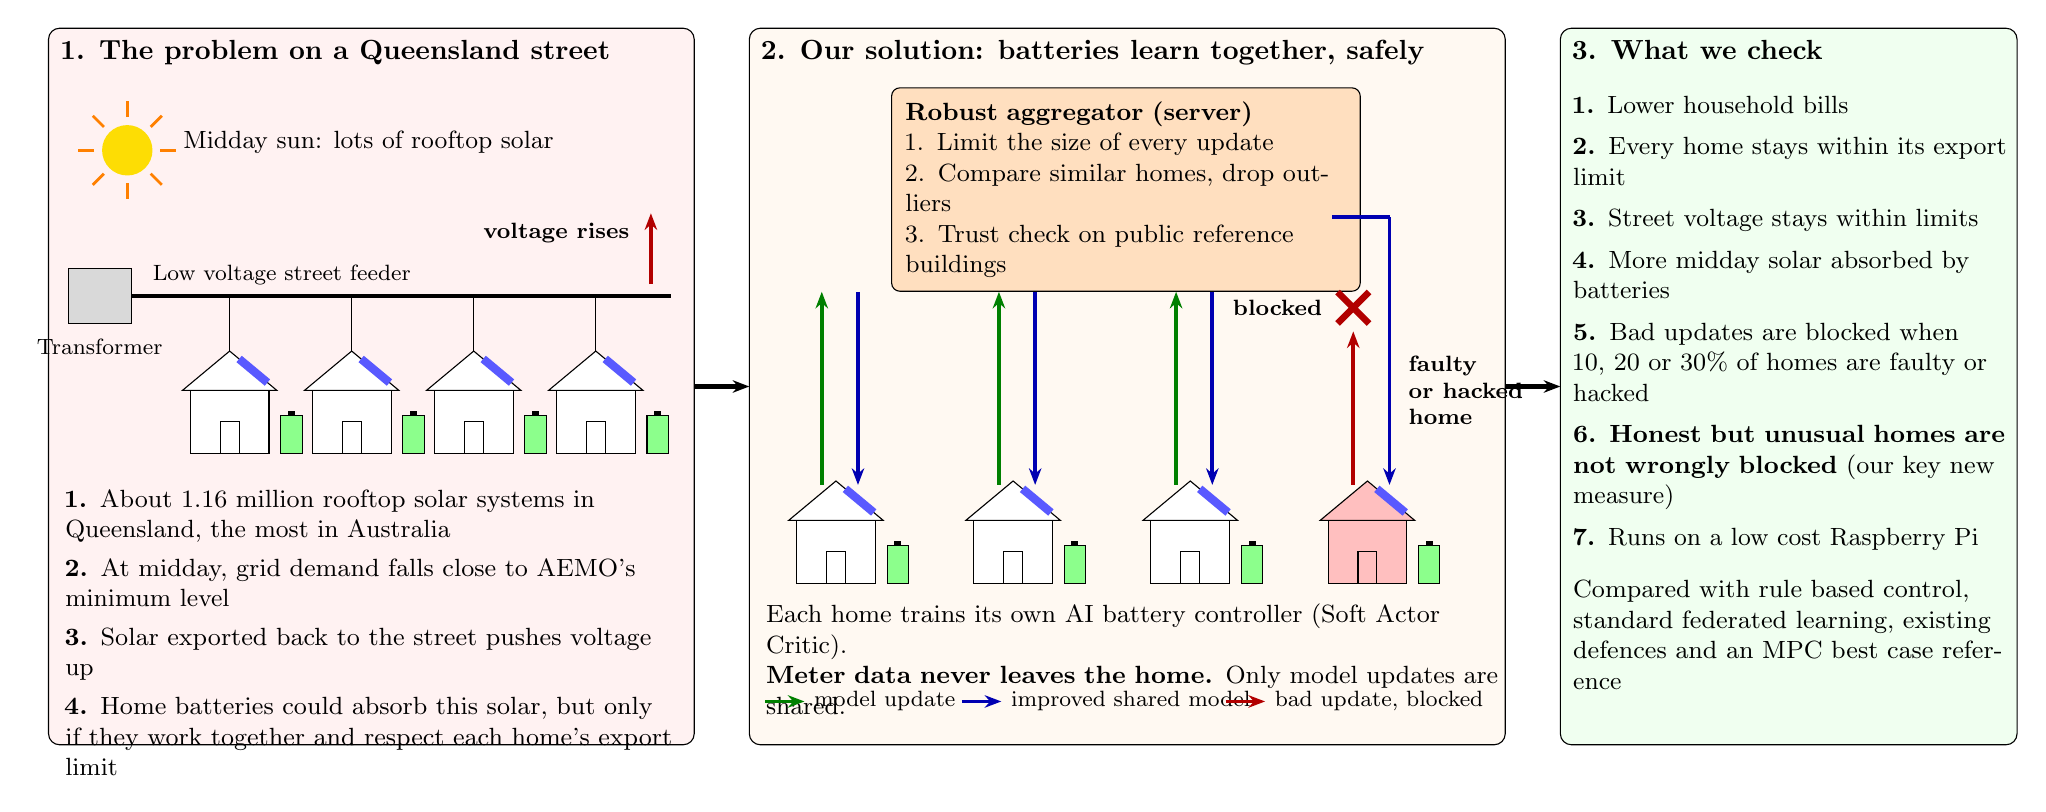
\begin{tikzpicture}[font=\fontsize{9}{11}\selectfont, text=black, >={Stealth[length=6pt]},
  txt/.style={anchor=north west, align=left, inner sep=3pt},
  ttl/.style={anchor=north west, align=left, inner sep=4pt, font=\fontsize{10}{12}\selectfont\bfseries}]
% house: #1 x, #2 y (bottom left), #3 wall fill
\def\house#1#2#3{%
  \draw[fill=#3] (#1,#2) rectangle (#1+1,#2+0.8);
  \draw[fill=#3] (#1-0.1,#2+0.8) -- (#1+0.5,#2+1.3) -- (#1+1.1,#2+0.8) -- cycle;
  \draw[line width=3pt, blue!65] (#1+0.62,#2+1.2) -- (#1+0.98,#2+0.9);
  \draw[fill=green!45] (#1+1.15,#2) rectangle (#1+1.42,#2+0.48);
  \fill (#1+1.24,#2+0.48) rectangle (#1+1.33,#2+0.54);
  \draw (#1+0.38,#2) rectangle (#1+0.62,#2+0.4);}


% ---------- Panel backgrounds ----------
\draw[rounded corners=4pt, fill=red!5]    (0,0)    rectangle (8.2,-9.1);
\draw[rounded corners=4pt, fill=orange!5] (8.9,0)  rectangle (18.5,-9.1);
\draw[rounded corners=4pt, fill=green!6]  (19.2,0) rectangle (25,-9.1);
\draw[->, line width=2pt] (8.2,-4.55) -- (8.9,-4.55);
\draw[->, line width=2pt] (18.5,-4.55) -- (19.2,-4.55);

% ---------- Panel 1: the problem ----------
\node[ttl] at (0,0) {1. The problem on a Queensland street};
% sun
\fill[yellow!80!orange] (1.0,-1.55) circle (0.32);
\foreach \a in {0,45,...,315} \draw[orange, line width=1pt] (1.0,-1.55) ++(\a:0.42) -- ++(\a:0.2);
\node[txt] at (1.6,-1.2) {Midday sun: lots of rooftop solar};
% transformer and feeder
\draw[fill=gray!30] (0.25,-3.75) rectangle (1.05,-3.05);
\node[font=\fontsize{8}{9.5}\selectfont, align=center] at (0.65,-4.05) {Transformer};
\draw[line width=1.4pt] (1.05,-3.4) -- (7.9,-3.4);
\node[anchor=south west, font=\fontsize{8}{9.5}\selectfont] at (1.2,-3.38) {Low voltage street feeder};
\foreach \x in {1.8,3.35,4.9,6.45} \draw (\x+0.5,-3.4) -- (\x+0.5,-4.1);
\house{1.8}{-5.4}{white}
\house{3.35}{-5.4}{white}
\house{4.9}{-5.4}{white}
\house{6.45}{-5.4}{white}
% voltage rise marker
\draw[->, red!70!black, line width=1.6pt] (7.65,-3.25) -- (7.65,-2.35);
\node[anchor=east, font=\fontsize{8}{9.5}\selectfont\bfseries, text=black] at (7.5,-2.6) {voltage rises};
\node[txt, text width=7.7cm] at (0.1,-5.75) {%
\textbf{1.} About 1.16 million rooftop solar systems in Queensland, the most in Australia\\[3pt]
\textbf{2.} At midday, grid demand falls close to AEMO's minimum level\\[3pt]
\textbf{3.} Solar exported back to the street pushes voltage up\\[3pt]
\textbf{4.} Home batteries could absorb this solar, but only if they work together and respect each home's export limit};

% ---------- Panel 2: our solution ----------
\node[ttl] at (8.9,0) {2. Our solution: batteries learn together, safely};
\node[draw, rounded corners=3pt, fill=orange!25, align=left, anchor=north west, text width=5.6cm, inner sep=5pt] (agg) at (10.7,-0.75) {%
\textbf{Robust aggregator (server)}\\
1. Limit the size of every update\\
2. Compare similar homes, drop outliers\\
3. Trust check on public reference buildings};
% houses
\house{9.5}{-7.05}{white}
\house{11.75}{-7.05}{white}
\house{14.0}{-7.05}{white}
\house{16.25}{-7.05}{red!25}
% arrows for honest homes
\foreach \x in {9.5,11.75,14.0} {
  \draw[->, green!50!black, line width=1.4pt] (\x+0.32,-5.8) -- (\x+0.32,0 |- agg.south);
  \draw[->, blue!70!black, line width=1.4pt] (\x+0.78,0 |- agg.south) -- (\x+0.78,-5.8);
}
% hacked home
\draw[->, red!70!black, line width=1.4pt] (16.57,-5.8) -- (16.57,-3.85);
\draw[red!70!black, line width=2.4pt] (16.37,-3.35) -- (16.77,-3.75) (16.37,-3.75) -- (16.77,-3.35);
\node[anchor=east, font=\fontsize{8}{9.5}\selectfont\bfseries] at (16.3,-3.55) {blocked};
\draw[->, blue!70!black, line width=1.4pt] (17.03,-2.4) -- (17.03,-5.8);\draw[blue!70!black, line width=1.4pt] (16.3,-2.4) -- (17.03,-2.4);
\node[anchor=west, font=\fontsize{8}{9.5}\selectfont\bfseries, align=left] at (17.15,-4.6) {faulty\\or hacked\\home};
\node[txt, text width=9.3cm] at (9.0,-7.2) {Each home trains its own AI battery controller (Soft Actor Critic).\\
\textbf{Meter data never leaves the home.} Only model updates are shared.};
% legend
\draw[->, green!50!black, line width=1.4pt] (9.1,-8.55) -- (9.6,-8.55);
\node[anchor=west, font=\fontsize{8}{9.5}\selectfont] at (9.6,-8.55) {model update};
\draw[->, blue!70!black, line width=1.4pt] (11.6,-8.55) -- (12.1,-8.55);
\node[anchor=west, font=\fontsize{8}{9.5}\selectfont] at (12.1,-8.55) {improved shared model};
\draw[->, red!70!black, line width=1.4pt] (14.95,-8.55) -- (15.45,-8.55);
\node[anchor=west, font=\fontsize{8}{9.5}\selectfont] at (15.45,-8.55) {bad update, blocked};

% ---------- Panel 3: what we check ----------
\node[ttl] at (19.2,0) {3. What we check};
\node[txt, text width=5.5cm] at (19.25,-0.75) {%
\textbf{1.} Lower household bills\\[4pt]
\textbf{2.} Every home stays within its export limit\\[4pt]
\textbf{3.} Street voltage stays within limits\\[4pt]
\textbf{4.} More midday solar absorbed by batteries\\[4pt]
\textbf{5.} Bad updates are blocked when 10, 20 or 30\% of homes are faulty or hacked\\[4pt]
\textbf{6.} \textbf{Honest but unusual homes are not wrongly blocked} (our key new measure)\\[4pt]
\textbf{7.} Runs on a low cost Raspberry Pi\\[8pt]
Compared with rule based control, standard federated learning, existing defences and an MPC best case reference};

\end{tikzpicture}%
}
\caption{FedGrid-RL overview: the Queensland problem, the robust federated learning solution, and what is evaluated.}
\label{fig:pipeline}
\end{figure}

\subsection{Queensland case study}
\begin{itemize}
  \item \textbf{Network.} A suburban low voltage feeder from the CSIRO National Low Voltage Feeder Taxonomy~\cite{csiro_lv}, with 20 to 50 homes, modelled in pandapower with three phase unbalanced power flow, since Australian low voltage streets are three phase. A second, larger CSIRO feeder is used to test scaling to about 100 homes.
  \item \textbf{Household data.} Load and solar profiles from the Ausgrid Solar Home Electricity Data~\cite{ausgrid}, with solar output rescaled to Toowoomba or Brisbane weather from the Bureau of Meteorology. Battery sizes follow typical Cheaper Home Batteries Program installations. This data comes from New South Wales homes between 2010 and 2013, and those homes had no batteries, so the Queensland rescaling is treated as a sensitivity test rather than a direct model of Queensland households.
  \item \textbf{Prices.} The Energex residential time of use network tariff~\cite{energex_tariff}, tariff 6900, which charges its lowest off peak rate from 11am to 4pm and its peak rate from 4pm to 9pm every day, plus AEMO Queensland wholesale prices as a second case.
  \item \textbf{Network rules.} Export limits follow a simple per phase schedule capped at 10\,kW, tightened for each home according to its voltage sensitivity on the feeder. Following Energex rules, each home keeps a minimum export of 1.5\,kW when limits are reduced and falls back to 1.5\,kW after a day without communication~\cite{energex_doe}. Computing full dynamic operating envelopes from optimal power flow is a research topic of its own and is left for later work. Minimum system load events are fixed scenarios on selected days, based on AEMO thresholds, during which exports are pushed towards zero.
\end{itemize}

\subsection{Learning setup}
Each home has one agent that uses Soft Actor Critic~\cite{haarnoja2018} in the CityLearn environment to decide when to charge and discharge the battery. CityLearn has no power flow model, so it will be coupled to pandapower at each time step. If this coupling proves too slow, a small Gym environment built around pandapower will be used instead. Each agent's network has a shared part, which is trained with all homes, and a small local part that stays in the home and adapts to that household. Agents train locally and send only updates of the shared part to an aggregator, using FedAvg and FedProx~\cite{li2020fedprox}. Export limits are enforced by limiting battery discharge. If solar alone is above the limit, the inverter curtails solar. The reward penalises electricity cost, curtailed solar, any remaining export breach and voltage outside limits.

\subsection{Faulty and compromised homes}
We assume that a share of homes may send wrong updates because of weak passwords, bad firmware, faulty meters or deliberate tampering. We test updates that are flipped, scaled or crafted to slip past defences~\cite{fang2025}, as well as false meter readings and false rewards. We also add normal communication faults such as lost and delayed messages, so that honest but unreliable homes are not treated as attackers. Finally, we test an adaptive attacker who knows the defence and shapes its updates to look honest, because a defence is only credible if it holds against such an attacker.

\subsection{Robust aggregation}
The aggregator uses three simple steps:
\begin{enumerate}
  \item Limit the size of every update so no single home can dominate.
  \item Group homes that behave similarly, using only the updates the aggregator already receives or coarse details given at sign up such as solar size band. Unusual updates are then removed within each group, not across all homes. Very small groups are merged with the nearest group so that each group has enough members.
  \item Give each group a trust weight. The aggregator computes its own update on public reference buildings and weights each group by how closely its update agrees with it, similar to FLTrust~\cite{cao2021fltrust}. A group made only of bad homes therefore gets a low weight. The reference buildings are CityLearn challenge buildings kept outside the federation, so the aggregator never needs data from participating homes.
\end{enumerate}

\subsection{Evaluation}
\begin{center}
\small
\begin{tabularx}{\linewidth}{@{}lX@{}}
\toprule
\textbf{Item} & \textbf{Plan} \\
\midrule
Baselines & Rule based control, local SAC, central SAC, FedAvg SAC, FedProx SAC~\cite{sumayli2026}, median, trimmed mean, Krum, FLTrust, FLAME, a TAFDRL style trust filter~\cite{sepehrzad2026}, and a model predictive control reference \\
Ablation & Each of the three aggregation steps removed in turn, to show what each one contributes \\
Generalisation & A second feeder with up to about 100 homes, and a second household dataset \\
Network metrics & DOE breaches, voltage violations, transformer loading, midday demand absorbed during minimum load events \\
Household metrics & Electricity bill and battery cycling \\
Security metrics & Loss in performance under each attack, rate of honest homes wrongly rejected \\
Device metrics & Training and decision time and memory on a Raspberry Pi, and on the UniSQ hardware in the loop platform if access is possible \\
Reliability & At least three random seeds per setting, with confidence intervals \\
\bottomrule
\end{tabularx}
\end{center}

\section{Datasets}

All datasets used in this project are free and public. None of them needs an application or a data agreement.

\begin{enumerate}[leftmargin=1.6em, itemsep=6pt]
\item \textbf{Street network (CSIRO LV feeders).}
\begin{itemize}
  \item Download the whole repository as a zip: \url{https://github.com/csiro-energy-systems/RepresentativeLVNetworks/archive/refs/heads/master.zip}
  \item Repository page: \url{https://github.com/csiro-energy-systems/RepresentativeLVNetworks}
  \item \textbf{Contents:} 23 representative Australian low voltage networks in OpenDSS format, in the \texttt{data} folder, plus a Python reader.
  \item \textbf{Report to cite:} \url{https://arena.gov.au/assets/2022/08/national-low-voltage-feeder-taxonomy-study.pdf} (DOI 10.25919/2tas-7213)~\cite{csiro_lv}.
\end{itemize}

\item \textbf{Household load and solar (Ausgrid Solar Home Electricity Data).}
\begin{itemize}
  \item Page: \url{https://www.ausgrid.com.au/Industry/Our-Research/Data-to-share/Solar-home-electricity-data}
  \item \textbf{What to download:} the three half hour zip files, one per year: July 2010 to June 2011, 2011 to 2012, and 2012 to 2013. They are listed under ``Related documents'' on the page.
  \item \textbf{Contents:} 300 homes, half hourly, with general consumption, controlled load and gross solar generation~\cite{ausgrid}.
  \item \textbf{Backup page:} \url{https://data.nsw.gov.au/data/dataset/solar-home-electricty-data}
\end{itemize}

\item \textbf{Wholesale prices and demand (AEMO, Queensland).}
\begin{itemize}
  \item One CSV per month, direct link pattern: \url{https://aemo.com.au/aemo/data/nem/priceanddemand/PRICE_AND_DEMAND_YYYYMM_QLD1.csv}
  \item \textbf{Example:} \url{https://aemo.com.au/aemo/data/nem/priceanddemand/PRICE_AND_DEMAND_202509_QLD1.csv}
  \item \textbf{Contents:} five minute Queensland total demand and price.
  \item All 12 months of 2025 give both price signals and real minimum demand days.
\end{itemize}

\item \textbf{Network tariffs.}
\begin{itemize}
  \item \textbf{Energex 2025--26 (Brisbane and south east Queensland):} \url{https://www.energex.com.au/__data/assets/pdf_file/0006/1651551/Energex-Network-Tariff-Guide-2025-26.pdf}~\cite{energex_tariff}
  \item \textbf{Energex 2026--27:} \url{https://www.energex.com.au/__data/assets/pdf_file/0011/2058077/Energex-Network-Tariff-Guide-2026-27.pdf}
  \item \textbf{Ergon Energy 2025--26:} \url{https://www.energex.com.au/__data/assets/pdf_file/0009/1651554/Ergon-Energy-Network-Tariff-Guide-2025-26.pdf}
  \item Toowoomba is in Ergon Energy's network area, not Energex's. A Toowoomba case study will use the Ergon tariff, and a Brisbane case study will use the Energex tariff. The location will be confirmed before the testbed is built.
\end{itemize}

\item \textbf{Weather and solar irradiance (to rescale the Sydney solar data to Queensland).}
\begin{itemize}
  \item \textbf{NASA POWER, free hourly irradiance and temperature, no account needed.} Example for Toowoomba, 2025: \url{https://power.larc.nasa.gov/api/temporal/hourly/point?parameters=ALLSKY_SFC_SW_DWN,T2M&community=RE&longitude=151.95&latitude=-27.56&start=20250101&end=20251231&format=CSV}
  \item \textbf{Open-Meteo, free hourly history:} \url{https://archive-api.open-meteo.com/v1/archive?latitude=-27.56&longitude=151.95&start_date=2025-01-01&end_date=2025-12-31&hourly=shortwave_radiation,temperature_2m&timezone=Australia%2FBrisbane}
  \item \textbf{Bureau of Meteorology, Toowoomba Airport station 041529:} daily solar exposure from Climate Data Online at \url{https://www.bom.gov.au/climate/data/}. The Bureau gives only daily values for free, so NASA POWER or Open-Meteo will be used for hourly values.
\end{itemize}

\item \textbf{Battery simulator data (CityLearn).}
\begin{itemize}
  \item Install with \texttt{pip install citylearn==3.0.2}. Datasets download automatically, or can be browsed at \url{https://github.com/intelligent-environments-lab/CityLearn/tree/master/data/datasets}
  \item \textbf{Datasets used:} \texttt{citylearn\_challenge\_2022\_phase\_all}, for the reference buildings that set the trust weights. The newer \texttt{citylearn\_three\_phase\_electrical\_service\_demo} will also be checked, since version 3 appears to include some phase level electrical modelling that could reduce the pandapower coupling work.
\end{itemize}

\item \textbf{Grid thresholds for minimum load scenarios (AEMO).}
\begin{itemize}
  \item \textbf{Minimum system load thresholds fact sheet:} \url{https://www.aemo.com.au/-/media/files/initiatives/der/managing-minimum-system-load/2025-spring-and-summer-minimum-system-load-thresholds-fact-sheet.pdf}~\cite{aemo_msl}
  \item \textbf{Quarterly Energy Dynamics Q3 2025, for the 2,790\,MW record:} \url{https://www.aemo.com.au/-/media/files/major-publications/qed/2025/qed-q3-2025.pdf}~\cite{aemo_q3}
\end{itemize}
\end{enumerate}

\textbf{Priority for November 2026:} items 1 and 2 (the feeder and the Ausgrid zip files), 12 months of item 3, and one year of NASA POWER weather. This is enough to build the testbed and run the first baselines.

\section{Expected outcomes}
\begin{itemize}
  \item \textbf{For distribution networks:} evidence on whether learned battery control keeps homes within their export limits and reduces voltage rise, without collecting meter data centrally.
  \item \textbf{For AEMO:} an estimate of how much midday demand coordinated home batteries can absorb during minimum load events, and how much of this is lost when some devices are compromised.
  \item \textbf{For households:} bill savings with private data kept at home.
  \item \textbf{For research:} a new robust aggregation method for household level FRL, and an open Queensland testbed that others can reuse.
  \item \textbf{Publications:} one Q1 journal paper, submitted by the end of May 2027 to Applied Energy, Energy and AI, the International Journal of Electrical Power and Energy Systems or IEEE Transactions on Smart Grid. A short conference paper (IEEE ISGT Asia 2027 or AUPEC 2027) is optional and will only be written if it does not delay the journal paper.
\end{itemize}

\section{Timeline}
\begin{center}
\small
\begin{tabularx}{\linewidth}{@{}lX@{}}
\toprule
\textbf{Period} & \textbf{Work} \\
\midrule
November 2026 & Prepare the Queensland data and set up the feeder model in pandapower with three phase power flow \\
December 2026 & Connect CityLearn to pandapower, add export limits and curtailment, run baselines without attacks and share first results (Objective 1) \\
January 2027 & Attack and defence study on standard methods, and start designing the new aggregation method (Objective 2) \\
February 2027 & Complete the new aggregation method, compare it with all baselines including the TAFDRL style filter, and run ablations (Objective 3) \\
March 2027 & Q1 strength tests: adaptive attacker, scaling to about 100 homes on a second feeder, and a second household dataset \\
April 2027 & Write the journal paper and release the code \\
May 2027 & Revise with supervisor feedback and submit to a Q1 journal \\
June to September 2027 & Respond to reviewer comments and revise \\
\bottomrule
\end{tabularx}
\end{center}

We will hold fortnightly online meetings and share code on GitHub and the draft on Overleaf.

\begin{thebibliography}{99}
\footnotesize
\setlength{\itemsep}{1pt}

\bibitem{cec2025} Clean Energy Council, ``Rooftop solar and storage report: July to December 2025,'' Clean Energy Council, Melbourne, Australia, Feb. 2026. [Online]. Available: \url{https://cleanenergycouncil.org.au/getmedia/16ed1cff-8ddb-423a-b3ad-3f9fa8e4d594/rooftop-solar-and-storage-biannual-report_july-december-2025.pdf}

\bibitem{aemo_q3} Australian Energy Market Operator, ``Rising renewable energy output offsets demand growth,'' media release, 30 Oct. 2025. [Online]. Available: \url{https://www.aemo.com.au/newsroom/media-release/rising-renewable-energy-output-offsets-demand-growth}. See also AEMO, ``Quarterly Energy Dynamics Q3 2025,'' Oct. 2025, \url{https://www.aemo.com.au/-/media/files/major-publications/qed/2025/qed-q3-2025.pdf}

\bibitem{aemo_msl} Australian Energy Market Operator, ``Minimum system load thresholds'' (Fact sheet: 2025 spring and summer minimum system load thresholds), Sep. 2025. [Online]. Available: \url{https://www.aemo.com.au/-/media/files/initiatives/der/managing-minimum-system-load/2025-spring-and-summer-minimum-system-load-thresholds-fact-sheet.pdf}

\bibitem{pm_batteries} A. Albanese and C. Bowen, ``Half a million cheaper home batteries bringing down bills for Australian homes and businesses,'' joint media release, Prime Minister of Australia, 14 Aug. 2026. [Online]. Available: \url{https://www.pm.gov.au/media/half-million-cheaper-home-batteries-bringing-down-bills-australian-homes-and-businesses}

\bibitem{energex_doe} Energex, ``About Dynamic Connections,'' Energex, Brisbane, Australia. [Online]. Available: \url{https://www.energex.com.au/our-services/connections/residential-and-commercial-connections/solar-connections-and-other-technologies/dynamic-connections-for-energy-exports/about-dynamic-connections}. Accessed: Oct. 2026.

\bibitem{ergon_doe} Ergon Energy Network, ``About Dynamic Connections,'' Ergon Energy, Townsville, Australia. [Online]. Available: \url{https://www.ergon.com.au/network/our-services/connections/residential-and-commercial-connections/solar-connections-and-other-technologies/dynamic-connections-for-energy-exports/about-dynamic-connections}. Accessed: Oct. 2026.

\bibitem{aemo_isp} Australian Energy Market Operator, ``2026 Integrated System Plan for the National Electricity Market,'' AEMO, Melbourne, Australia, 25 Jun. 2026. [Online]. Available: \url{https://www.aemo.com.au/-/media/files/major-publications/isp/2026/2026-integrated-system-plan-isp.pdf}

\bibitem{homeaffairs_web} Department of Home Affairs, ``Security Standards for Smart Devices,'' Australian Government. [Online]. Available: \url{https://www.homeaffairs.gov.au/about-us/our-portfolios/cyber-security/security-standards-for-smart-devices}. Accessed: Oct. 2026.

\bibitem{homeaffairs} Department of Home Affairs, ``Cyber Security Legislative Reforms. Explanatory Document: Cyber Security (Security Standards for Smart Devices) Rules,'' Commonwealth of Australia, Canberra, 2024. [Online]. Available: \url{https://www.cisc.gov.au/resources-subsite/Documents/cyber-security-security-standards-for-smart-devices-explanatory-document.pdf}

\bibitem{sievers2025} J. Sievers, P. Henrich, M. Beichter, R. Mikut, V. Hagenmeyer, T. Blank, and F. Simon, ``Federated reinforcement learning for sustainable and cost-efficient energy management,'' \emph{Energy and AI}, vol.~21, Art. no. 100521, Sep. 2025, doi: 10.1016/j.egyai.2025.100521.

\bibitem{sumayli2026} M. Sumayli and O. M. Anubi, ``Federated Reinforcement Learning for Peak Demand Mitigation in Residential Energy Systems With Dynamic Comfort Preferences,'' \emph{IEEE Access}, vol.~14, pp.~8174--8187, 2026, doi: 10.1109/ACCESS.2026.3653933.

\bibitem{feng2024} B. Feng, H. Xu, G. Huang, Z. Liu, C. Guo, and Z. Chen, ``Byzantine-Resilient Economical Operation Strategy Based on Federated Deep Reinforcement Learning for Multiple Electric Vehicle Charging Stations Considering Data Privacy,'' \emph{J. Mod. Power Syst. Clean Energy}, vol.~12, no.~6, pp.~1957--1967, 2024, doi: 10.35833/MPCE.2023.000850.

\bibitem{sepehrzad2026} R. Sepehrzad, H. Hosseinalibeiki, N. Taghinezhad, N. Khosravi, A. Al Durra, and M. S. Sadabadi, ``Enhanced cyber-resilience in flexible energy markets for microgrids: A trust-aware federated deep reinforcement learning framework,'' \emph{Applied Energy}, vol.~406, Art. no. 127282, Mar. 2026, doi: 10.1016/j.apenergy.2025.127282.

\bibitem{peivand2026} A. Peivand and S. M. Nosratabadi, ``Byzantine-Resilient Federated Multi-Agent Optimization Framework for Cyber-Secure Interconnected Microgrids,'' arXiv:2606.19080v2 [eess.SY], Aug. 2026, doi: 10.48550/arXiv.2606.19080.

\bibitem{zhang2026survey} Z. Zhang, S. Rath, J. Xu, and T. Xiao, ``Federated Learning for Smart Grid: A Survey on Applications and Potential Vulnerabilities,'' \emph{ACM Trans. Cyber-Phys. Syst.}, vol.~10, no.~1, Art. no. 11, pp.~11:1--11:26, 2026, doi: 10.1145/3760788.

\bibitem{csiro_lv} F. Geth, T. S. Brinsmead, S. West, P. Goldthorpe, B. Spak, G. Cross, and J. Braslavsky, ``National Low-Voltage Feeder Taxonomy Study,'' CSIRO, Newcastle, Australia, 2021 (public release v1.1.2). [Online]. Available: \url{https://arena.gov.au/assets/2022/08/national-low-voltage-feeder-taxonomy-study.pdf}. Network models: CSIRO Energy Systems, ``RepresentativeLVNetworks,'' GitHub repository, \url{https://github.com/csiro-energy-systems/RepresentativeLVNetworks}

\bibitem{ausgrid} E. L. Ratnam, S. R. Weller, C. M. Kellett, and A. T. Murray, ``Residential load and rooftop PV generation: an Australian distribution network dataset,'' \emph{Int. J. Sustain. Energy}, vol.~36, no.~8, pp.~787--806, 2017, doi: 10.1080/14786451.2015.1100196. Dataset: Ausgrid, ``Solar home electricity data.'' [Online]. Available: \url{https://data.nsw.gov.au/data/dataset/solar-home-electricty-data}

\bibitem{energex_tariff} Energex, ``Energex Network Tariff Guide: 01 July 2025 to 30 June 2026,'' Energex, Brisbane, Australia, 2025. [Online]. Available: \url{https://www.energex.com.au/__data/assets/pdf_file/0006/1651551/Energex-Network-Tariff-Guide-2025-26.pdf}

\bibitem{haarnoja2018} T. Haarnoja, A. Zhou, P. Abbeel, and S. Levine, ``Soft Actor-Critic: Off-Policy Maximum Entropy Deep Reinforcement Learning with a Stochastic Actor,'' in \emph{Proc. 35th Int. Conf. Mach. Learn. (ICML)}, ser. Proc. Mach. Learn. Res., vol.~80, Stockholm, Sweden, 2018, pp.~1861--1870.

\bibitem{li2020fedprox} T. Li, A. K. Sahu, M. Zaheer, M. Sanjabi, A. Talwalkar, and V. Smith, ``Federated Optimization in Heterogeneous Networks,'' in \emph{Proc. Mach. Learn. Syst. (MLSys)}, I. Dhillon, D. Papailiopoulos, and V. Sze, Eds., vol.~2, Austin, TX, USA, 2020, pp.~429--450.

\bibitem{fang2025} M. Fang, X. Wang, and N. Z. Gong, ``Provably Robust Federated Reinforcement Learning,'' in \emph{Proc. ACM Web Conf. 2025 (WWW '25)}, Sydney, NSW, Australia, 2025, pp.~896--909, doi: 10.1145/3696410.3714728.

\bibitem{cao2021fltrust} X. Cao, M. Fang, J. Liu, and N. Z. Gong, ``FLTrust: Byzantine-robust Federated Learning via Trust Bootstrapping,'' in \emph{Proc. Netw. Distrib. Syst. Secur. Symp. (NDSS)}, Virtual, 2021, doi: 10.14722/ndss.2021.24434.

\end{thebibliography}

\end{document}
